\documentclass[border=4pt]{standalone}
\usepackage{tikz}
\usetikzlibrary{shapes.symbols,positioning,arrows.meta}

\begin{document}
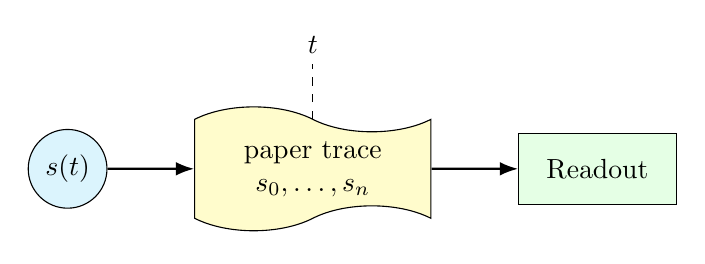
\begin{tikzpicture}[
  >=Latex,
  node distance=11mm,
  sensor/.style={draw,circle,minimum size=10mm,fill=cyan!14},
  strip/.style={tape,draw,tape bend top=out and in,
    tape bend bottom=in and out,tape bend height=9pt,
    minimum width=30mm,minimum height=13mm,fill=yellow!20,align=center},
  block/.style={draw,minimum width=20mm,minimum height=9mm,fill=green!10}
]
  \node[sensor] (sensor) {$s(t)$};
  \node[strip,right=of sensor] (record) {paper trace\\$s_0,\ldots,s_n$};
  \node[block,right=of record] (readout) {Readout};
  \draw[->,thick] (sensor) -- (record);
  \draw[->,thick] (record) -- (readout);
  \draw[dashed] (record.north) -- ++(0,7mm) node[above] {$t$};
\end{tikzpicture}
\end{document}
